\Aufgabe[e]{Isolines and isosurfaces} {
\begin{abc}
\item Sketch (if possible) the isolines of the following multivariate functions for the levels 0, 1 and -1:
\begin{iii}
\begin{multicols}{2}
\item $f_1(x,y)=xy,$
\item $f_2(x,y)=x^2y,$
\item $f_3(x,y)=xy^2,$
\item $f_4(x,y)=x^2y^2.$
\end{multicols}
\end{iii}
\item Given the multivariate function
$$f_5(x,y,z)=x^2+y^2-z.$$
Sketch the intersections of
\begin{iii}
\item the planes $z=0$, $z=1$, $z=-1$ with its isosurface of level 1,
\item the plane $z=2x+2y$ with its isosurface of level -1.
\end{iii}
\end{abc}
}


\Loesung{
\textbf{a)} 
\begin{iii}
\item The isolines of $f_1(x,y) = xy$ are pictured in figure \ref{f_1}.
\item The isolines of $f_2(x,y) = x^2y$ are pictured in figure \ref{f_2}.
\item The isolines of $f_3(x,y) = xy^2$ are pictured in figure \ref{f_3}.
\item The isolines of $f_4(x,y) = x^2y^2$ are pictured in figure \ref{f_4}. 
It is $f_4 \geq 0$ because $f_4$ is quadratic in $x$ and $y$. Therfore there is no isoline for the level -1.
\end{iii}
%\begin{figure}[ht]
%\begin{center}
%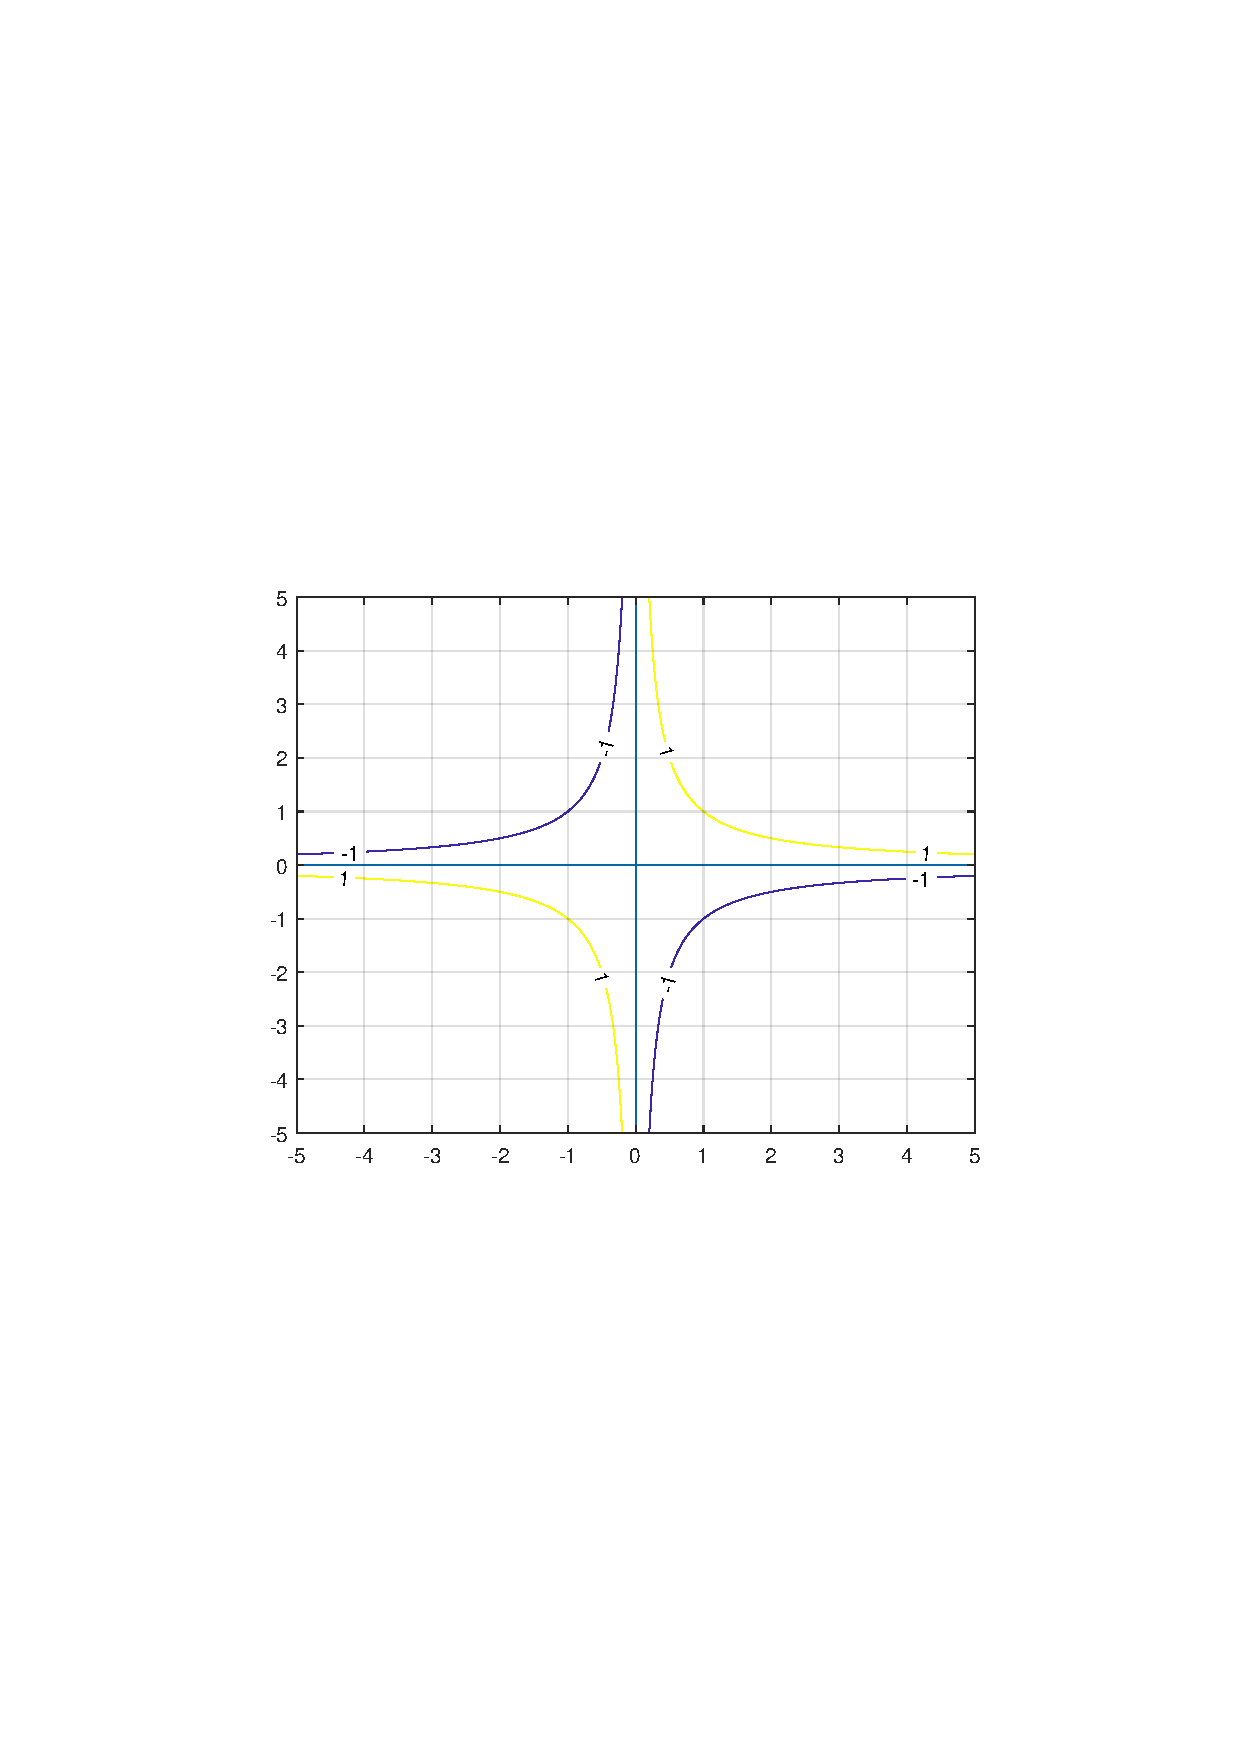
\includegraphics[width=15cm, height=15cm]{../A/analysis/isolines_and_isosurfaces_001_ai.pdf}
%\caption{Isolines of $f_1(x,y) = xy$.}
%\label{f_1}
%\end{center}
%\end{figure}
%
%\begin{figure}[ht]
%\begin{center}
%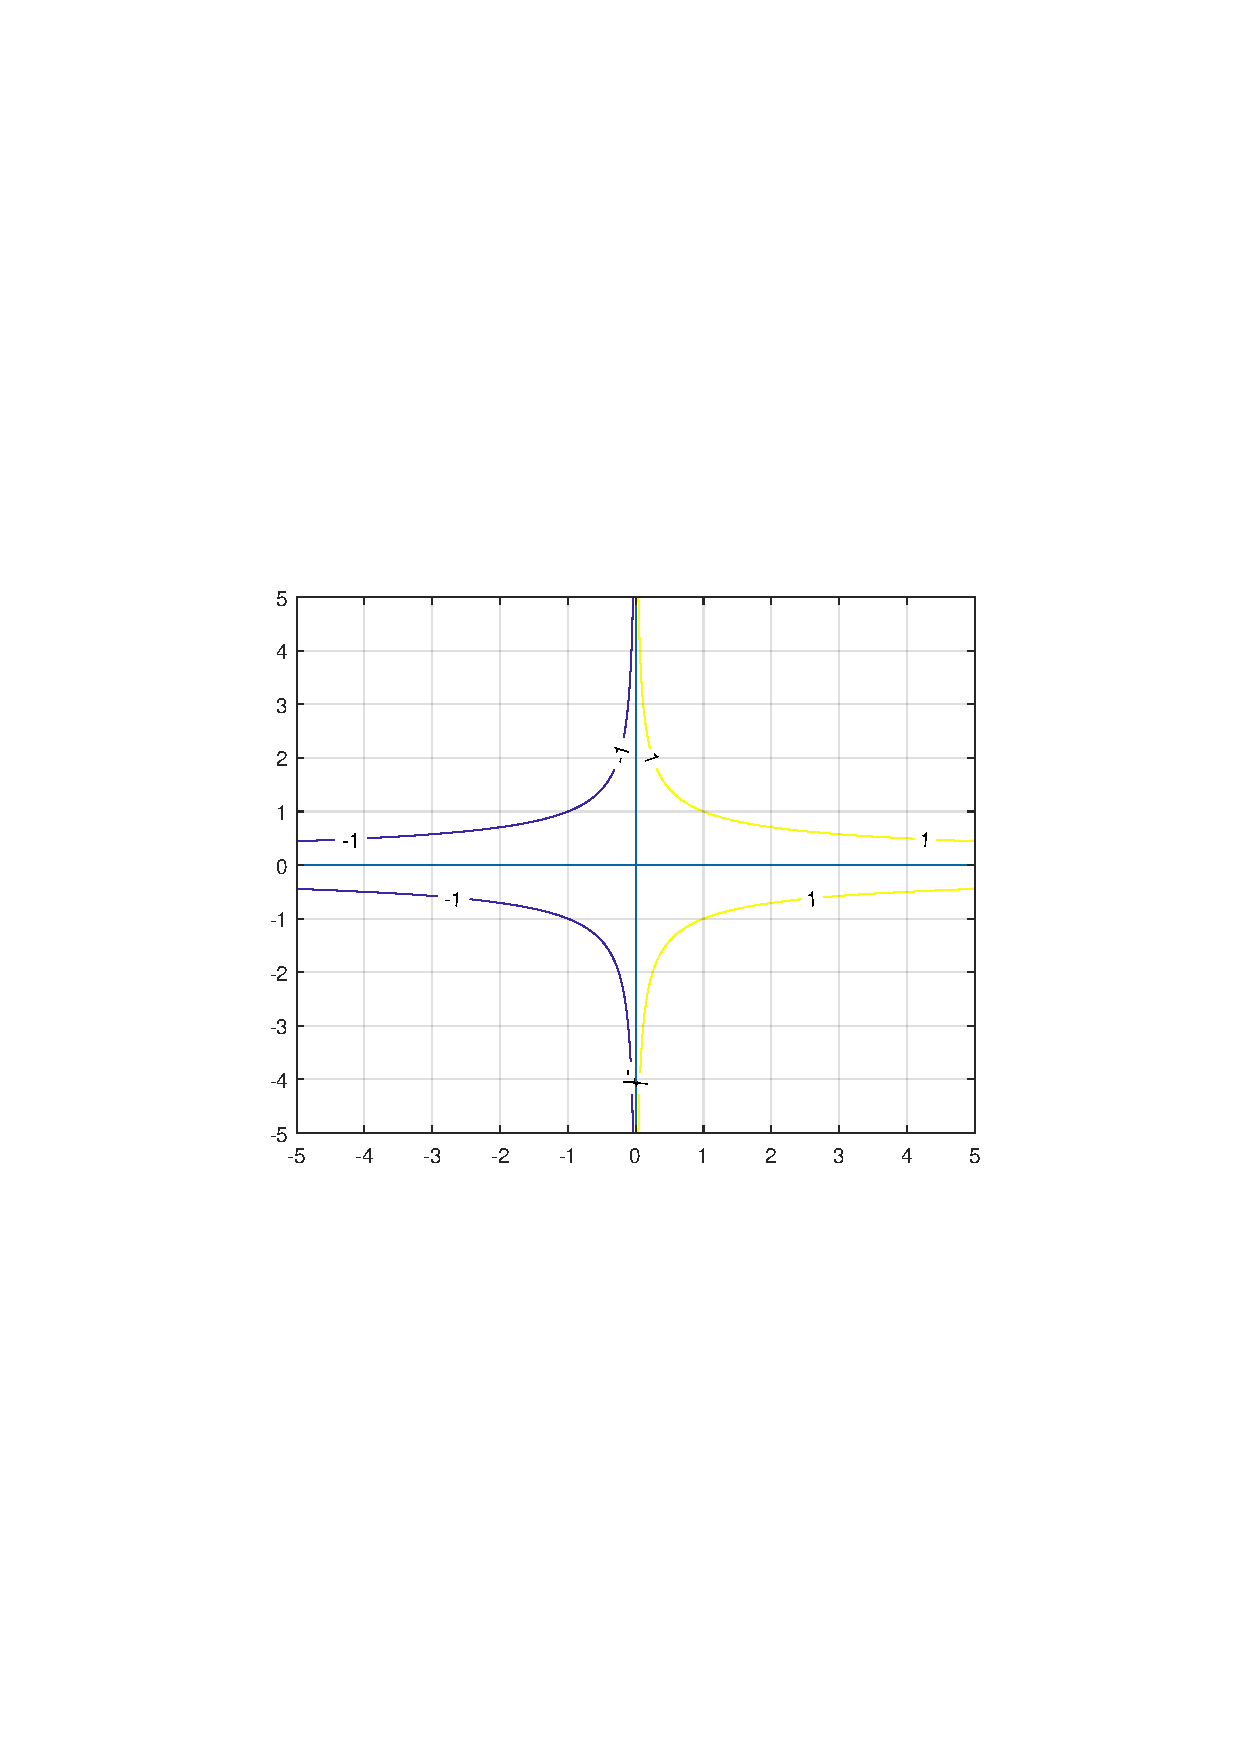
\includegraphics[width=15cm, height=15cm]{../A/analysis/isolines_and_isosurfaces_001_aii.pdf}
%\caption{Isolines of $f_2(x,y) = x^2y$.}
%\label{f_2}
%\end{center}
%\end{figure}
%
%\begin{figure}[ht]
%\begin{center}
%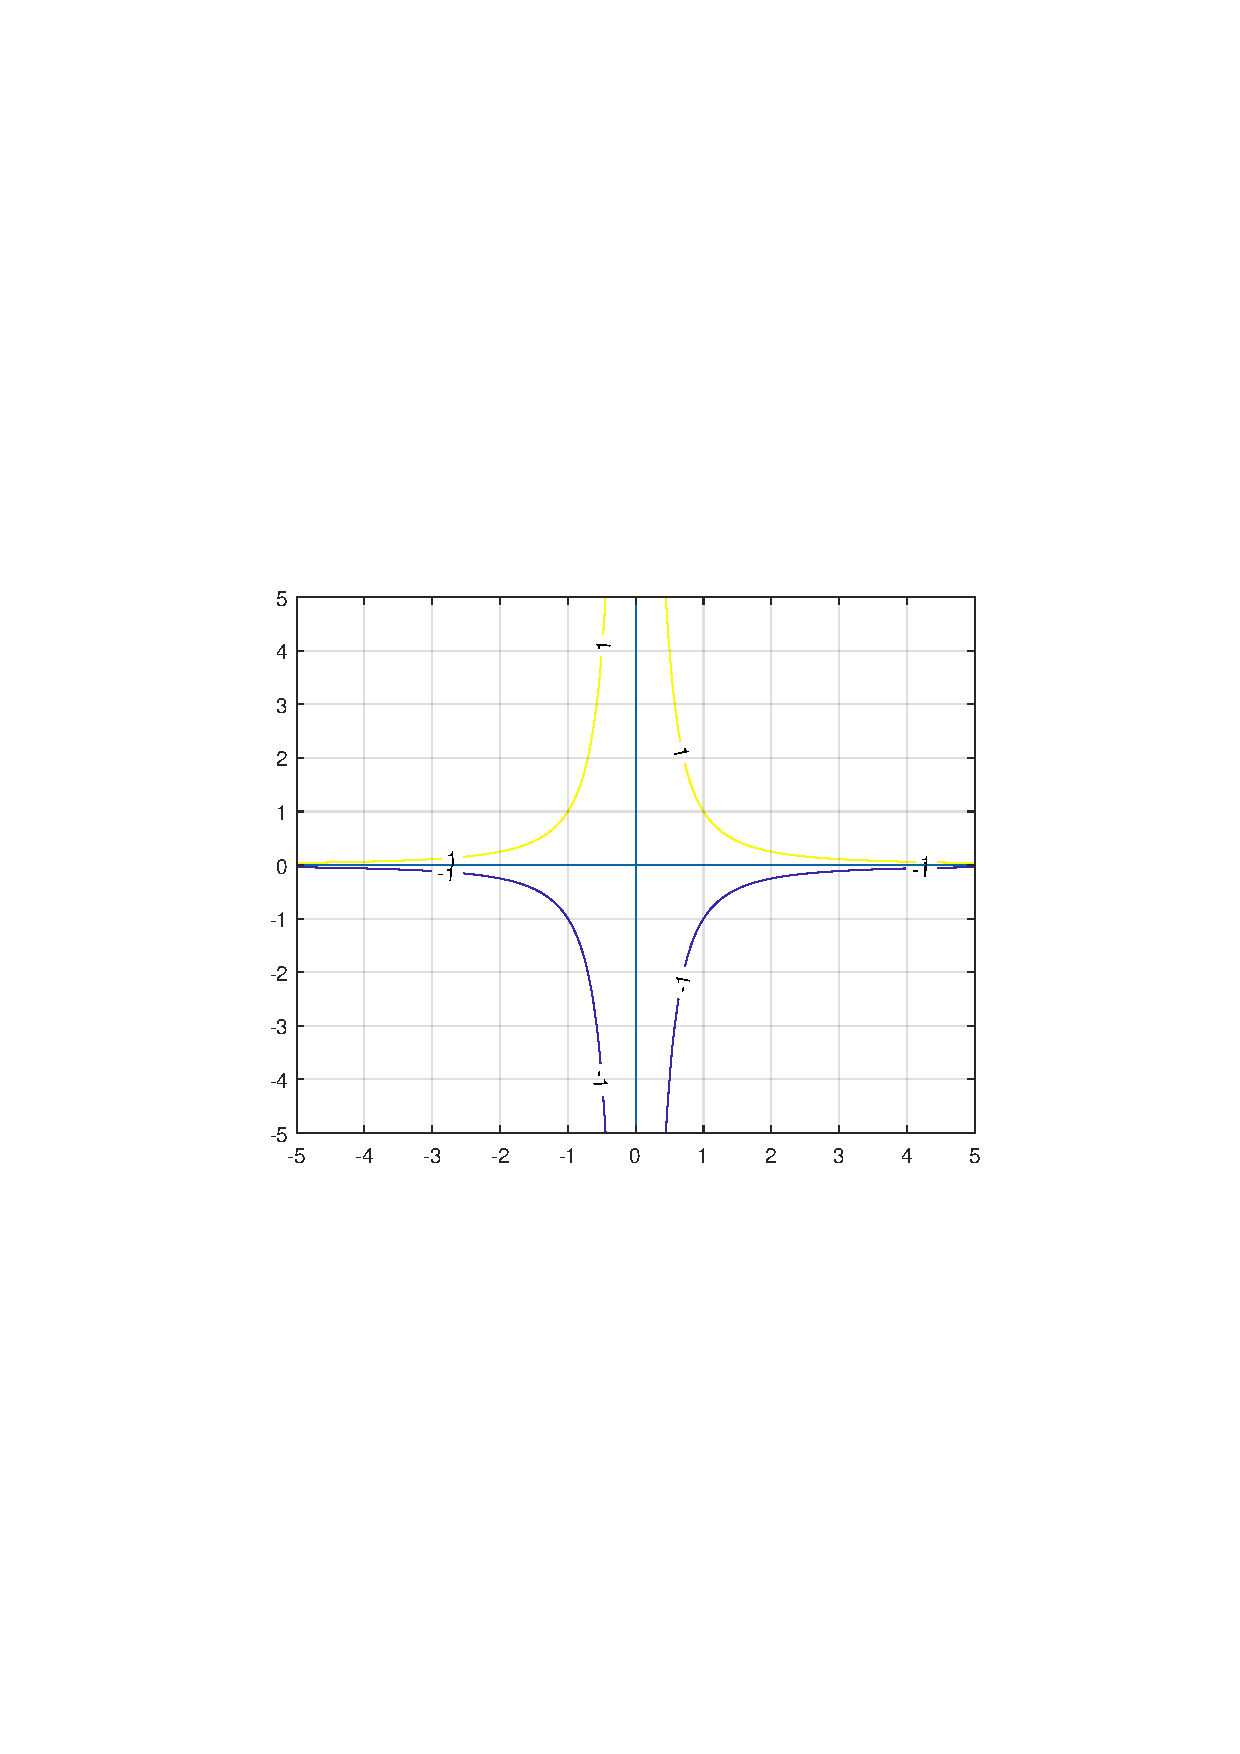
\includegraphics[width=15cm, height=15cm]{../A/analysis/isolines_and_isosurfaces_001_aiii.pdf}
%\caption{Isolines of $f_3(x,y) = xy^2$.}
%\label{f_3}
%\end{center}
%\end{figure}
%
%\begin{figure}[ht]
%\begin{center}
%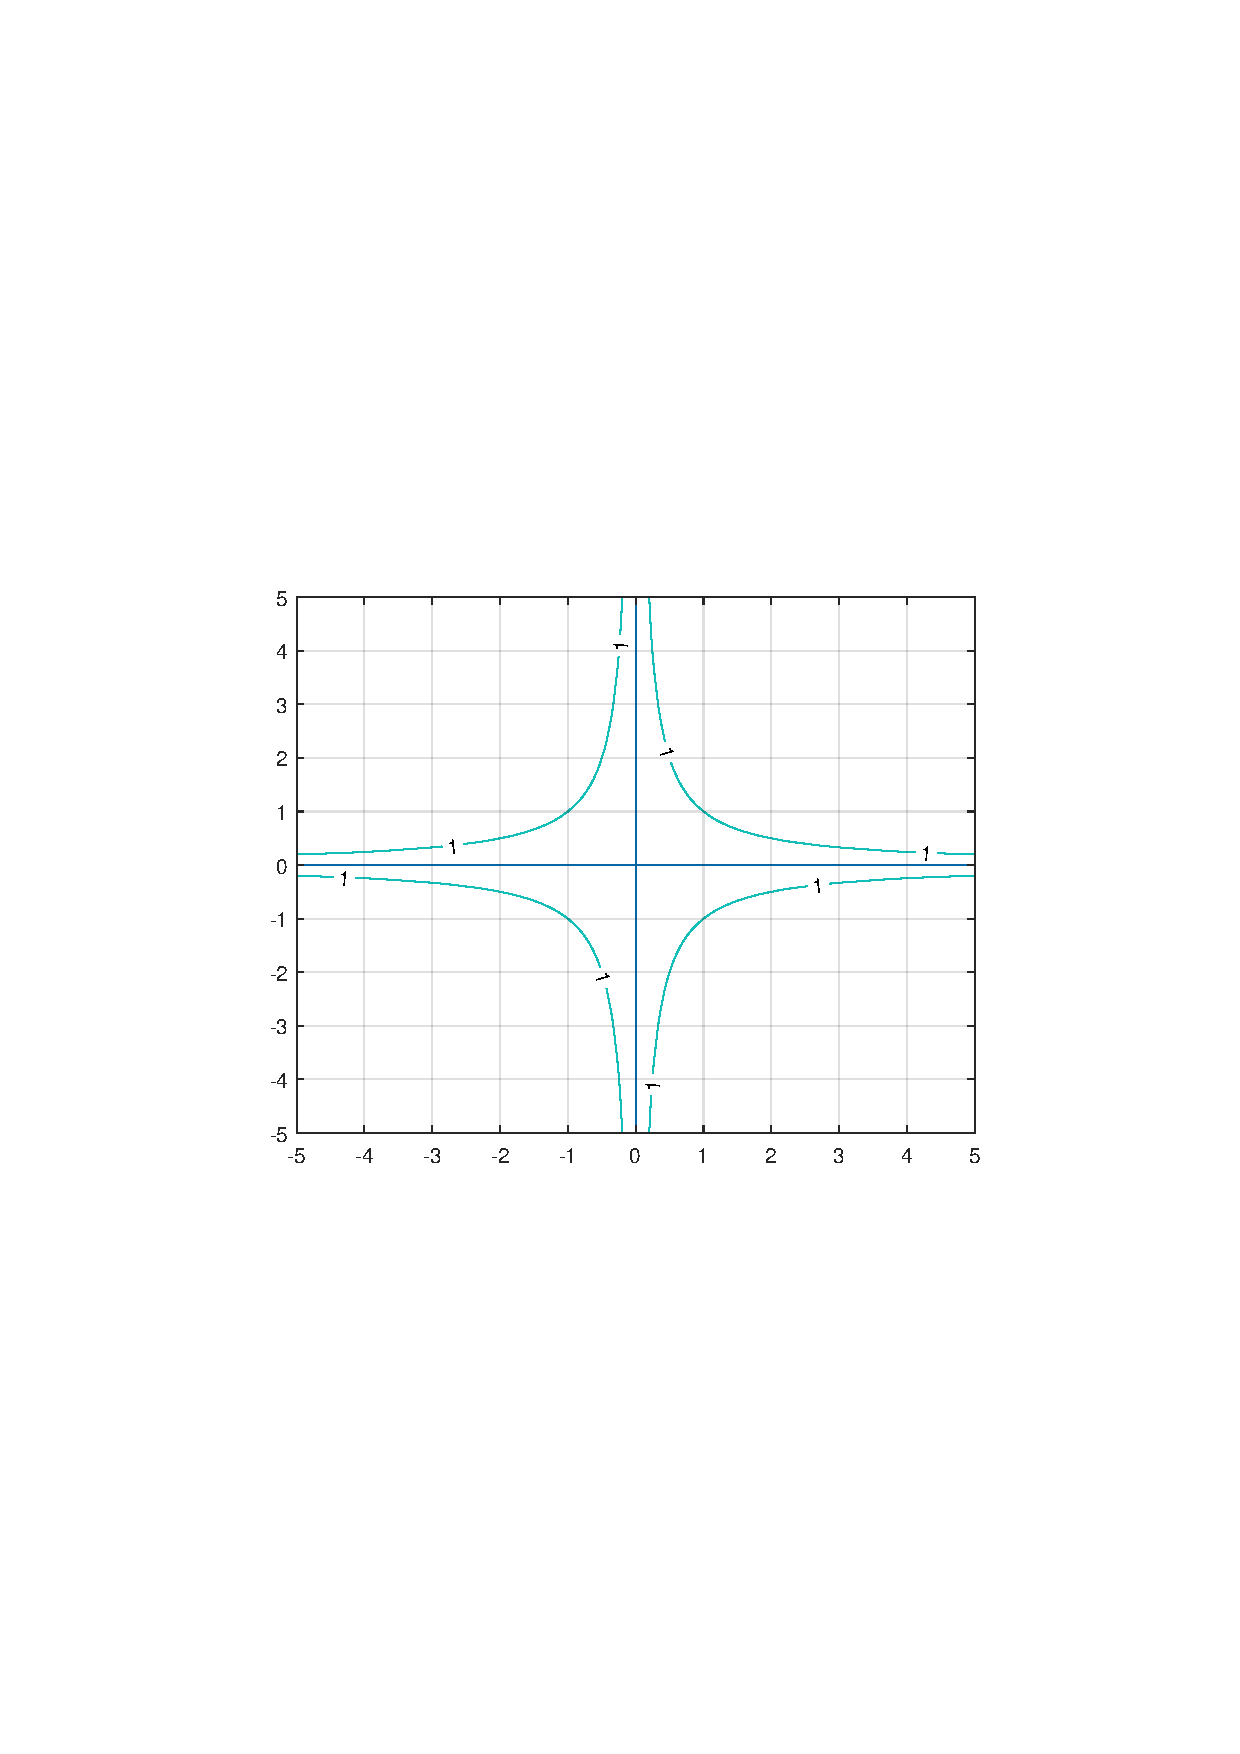
\includegraphics[width=15cm, height=15cm]{../A/analysis/isolines_and_isosurfaces_001_aiv.pdf}
%\caption{Isolines of $f_4(x,y) = x^2y^2$.}
%\label{f_4}
%\end{center}
%\end{figure}


\textbf{b)}
\begin{iii}
\item The function $f_5$ is a paraboloid. The intersection with the plane $z = 0$ is a circle with the radius 1 (see figure \ref{z=0}).\\
The intersection with the plane $z = 1$ is a circle with the radius $\sqrt{2}$ (see figure \ref{z=1}). 
The intersection with the plane $z = -1$ is the point at $(0,0)$ (see figure \ref{z=-1}). 
\item The intersection of the function $f_5$ and the plane $z =2x+2y$ is an ellipse (see figure \ref{z=2x+2y}).
\end{iii}
%\begin{figure}[ht]
%\begin{center}
%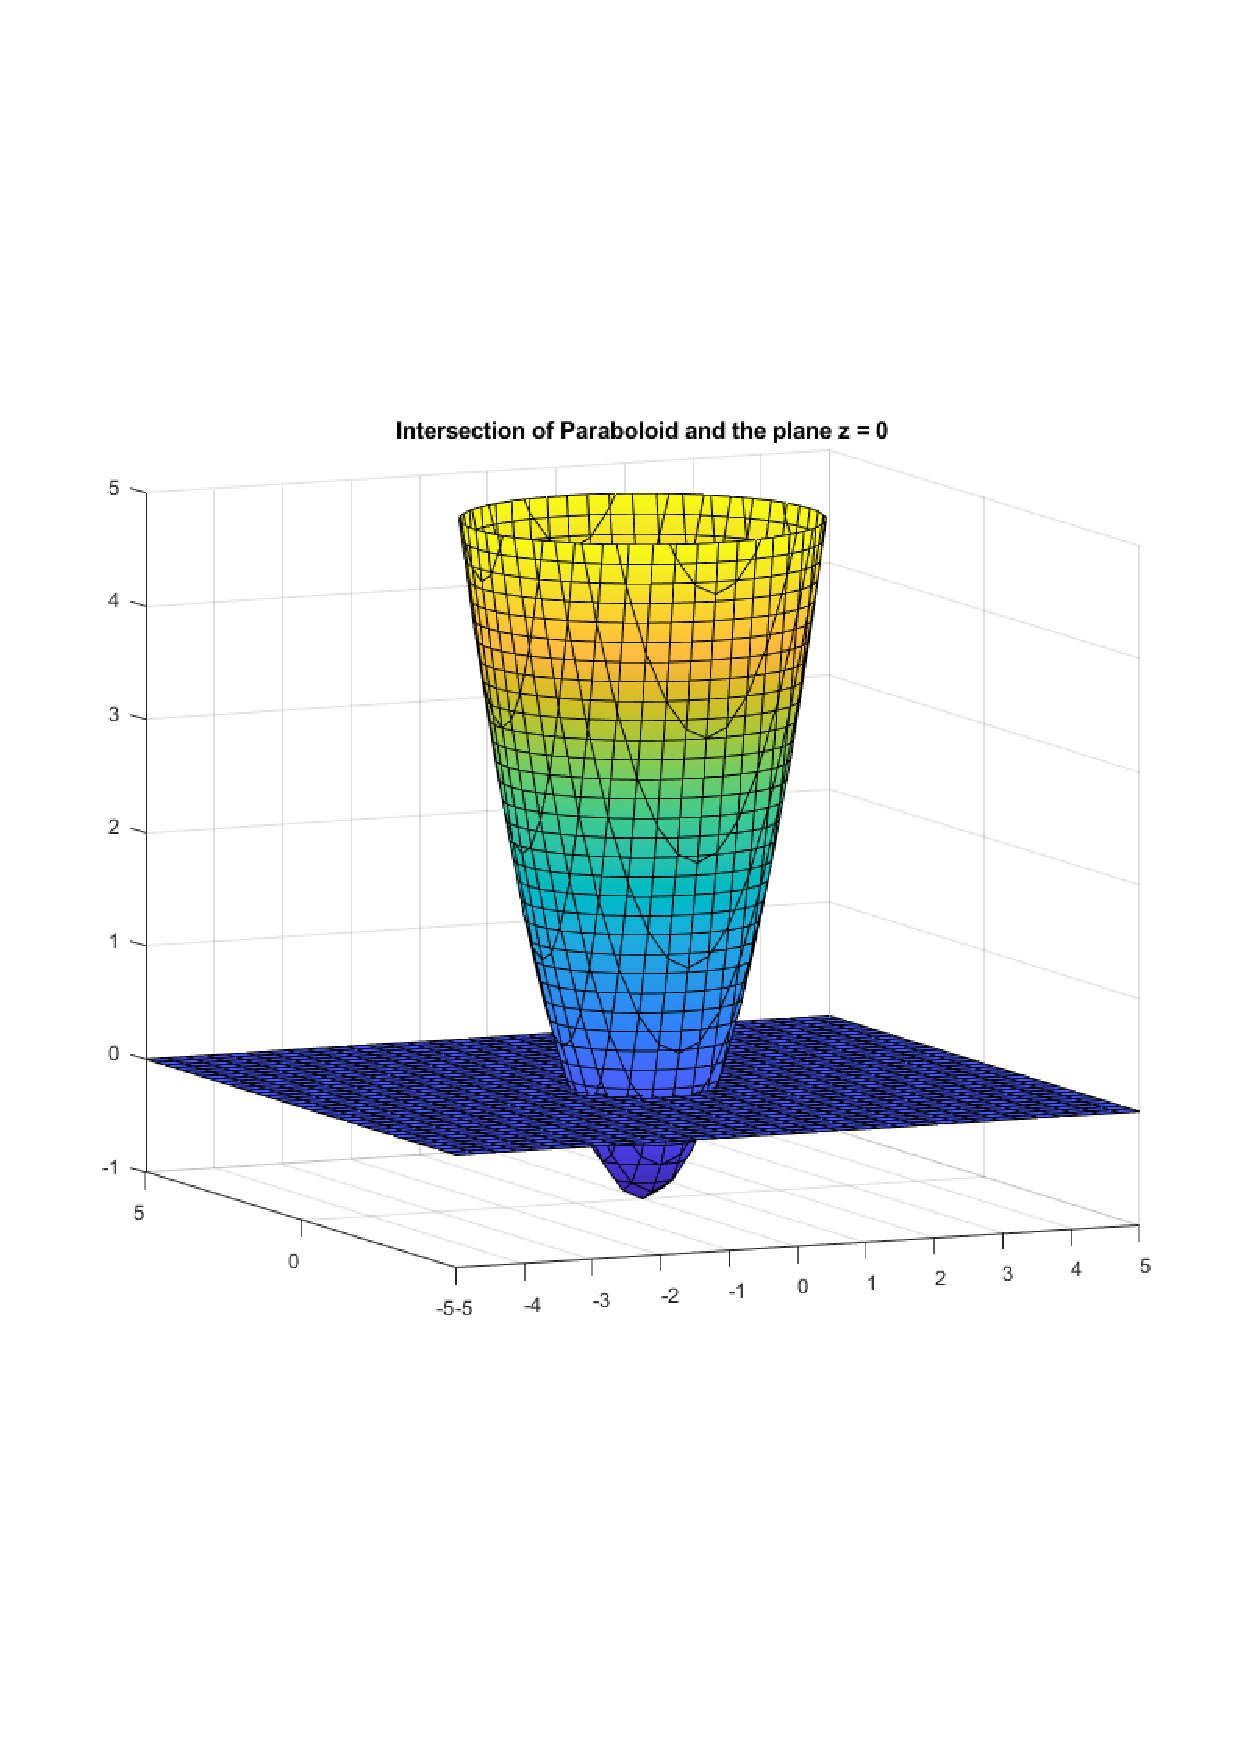
\includegraphics[width=15cm, height=15cm]{../A/analysis/isolines_and_isosurfaces_001_bi1.pdf}
%\caption{Intersection of the paraboloid and the plane $z=0$.}
%\label{z=0}
%\end{center}
%\end{figure}
%
%\begin{figure}[ht]
%\begin{center}
%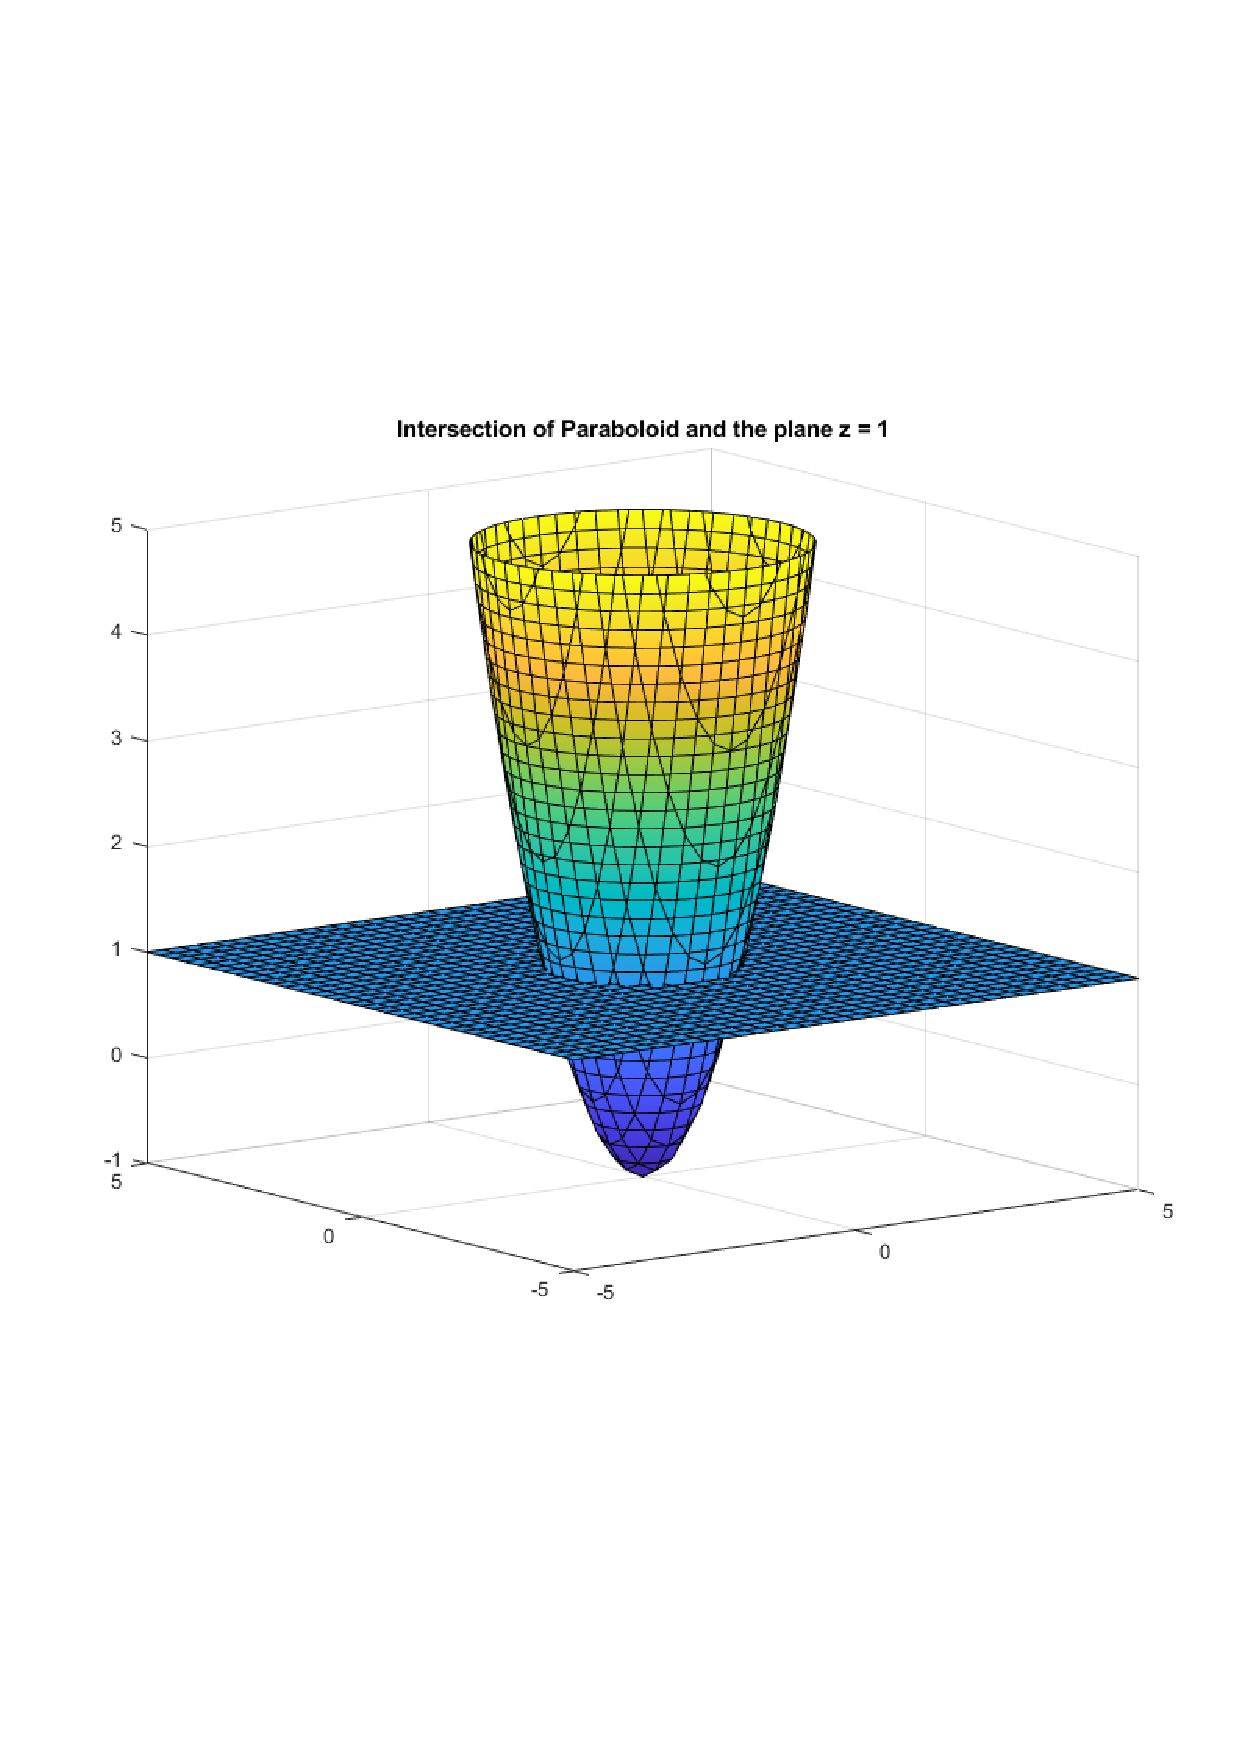
\includegraphics[width=15cm, height=15cm]{../A/analysis/isolines_and_isosurfaces_001_bi2.pdf}
%\caption{Intersection of the paraboloid and the plane $z=1$.}
%\label{z=1}
%\end{center}
%\end{figure}
%
%\begin{figure}[ht]
%\begin{center}
%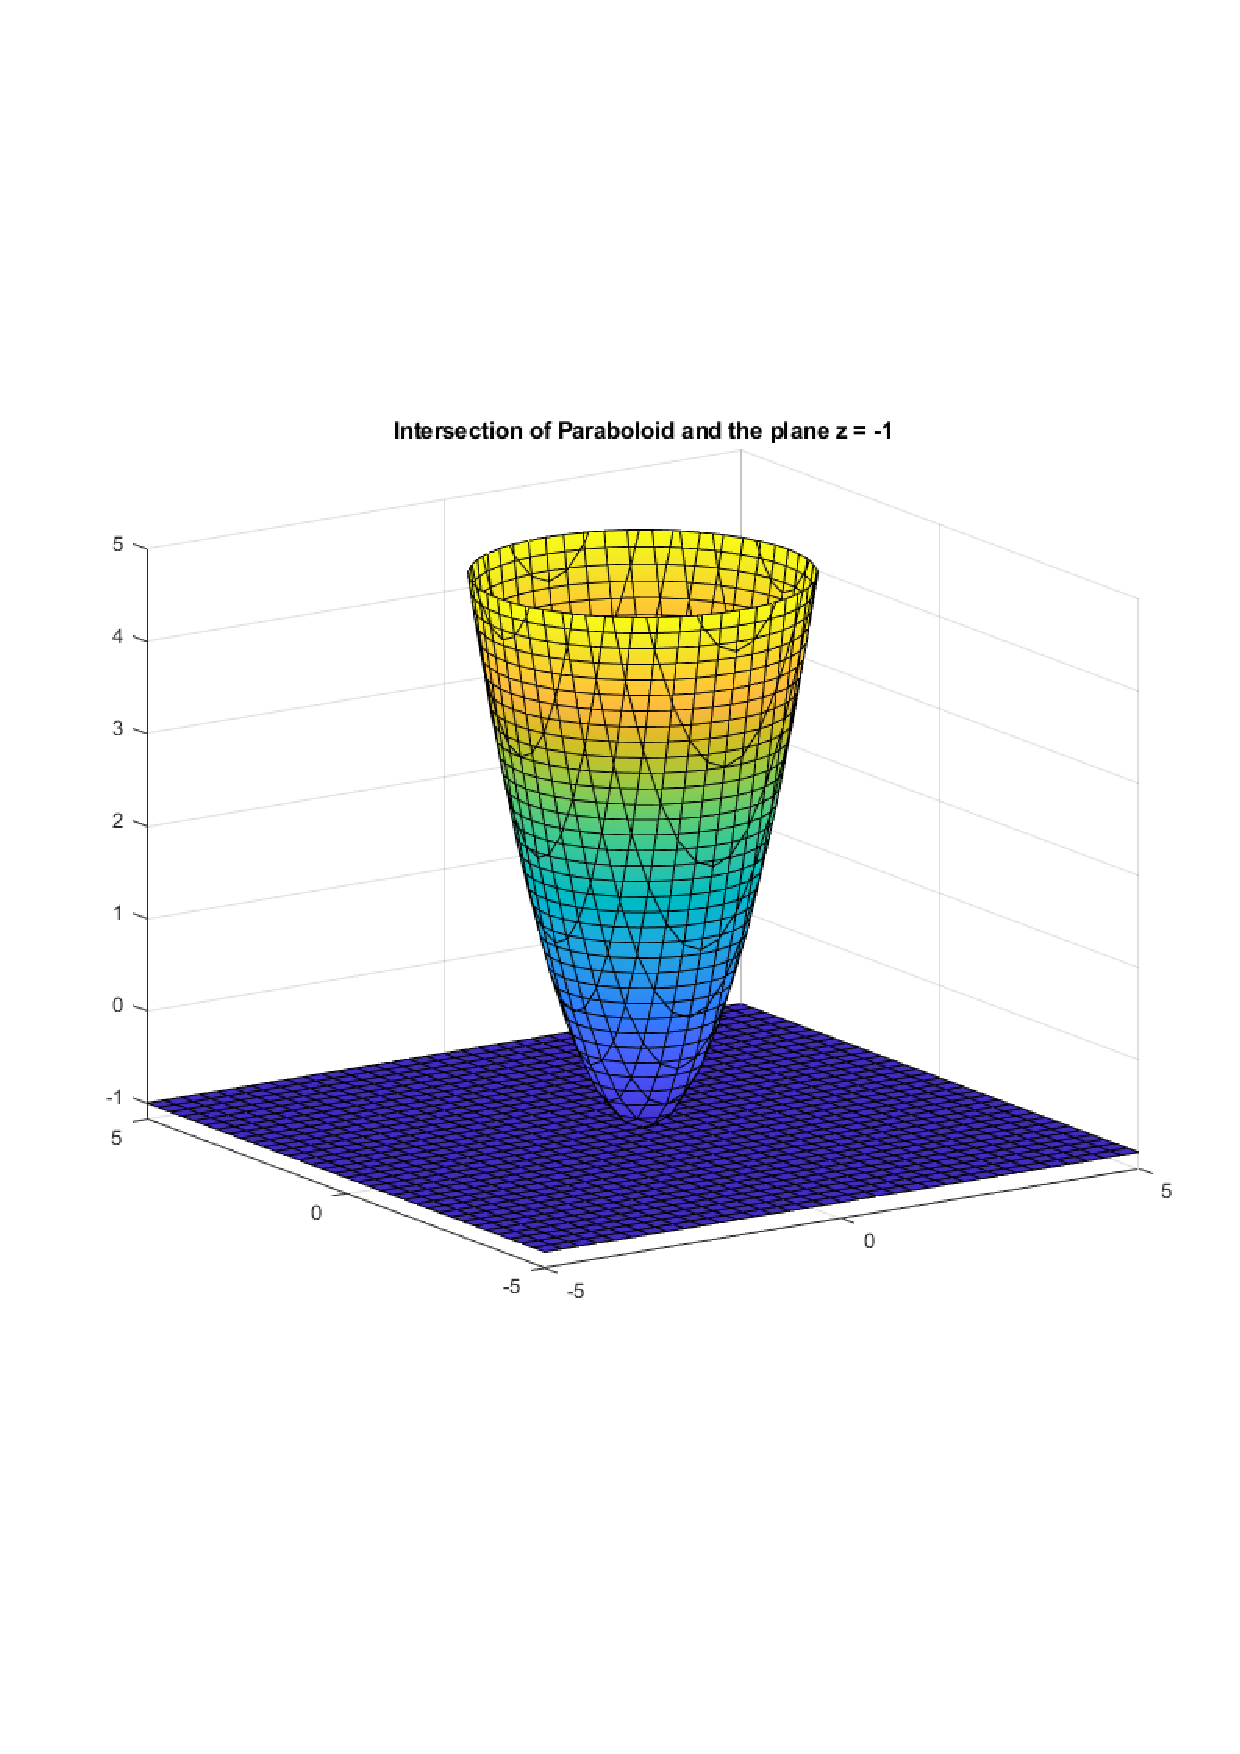
\includegraphics[width=15cm, height=15cm]{../A/analysis/isolines_and_isosurfaces_001_bi3.pdf}
%\caption{Intersection of the paraboloid and the plane $z=-1$.}
%\label{z=-1}
%\end{center}
%\end{figure}
%
%\begin{figure}[ht]
%\begin{center}
%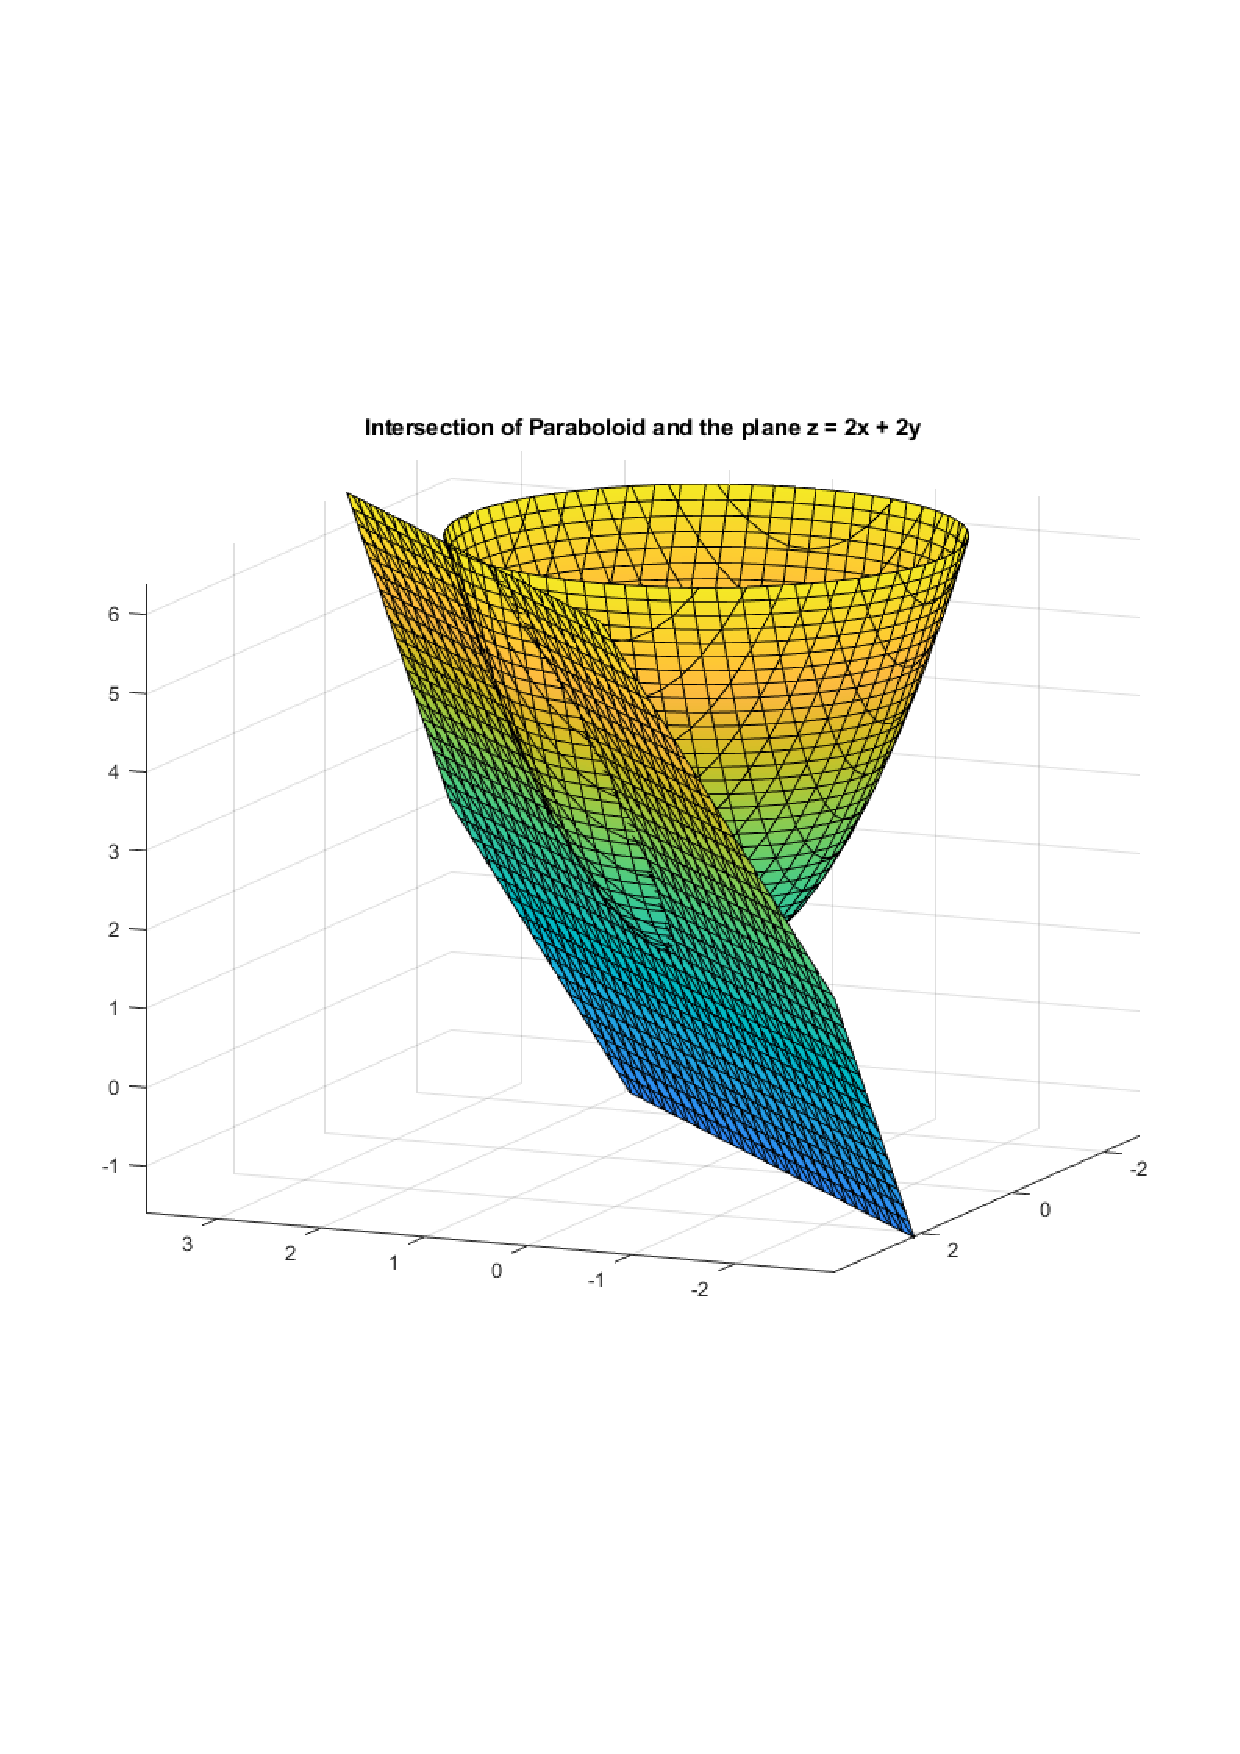
\includegraphics[width=15cm, height=15cm]{../A/analysis/isolines_and_isosurfaces_001_bii.pdf}
%\caption{Intersection of the paraboloid and the plane $z=2x+2y$.}
%\label{z=2x+2y}
%\end{center}
%\end{figure}


}

